\chapter{Implementation}\label{sec:implementation}

In diesem Kapitel wird die Umsetzung der beiden in Kapitel \ref{sec:concept} erarbeiteten Konzepte vorgestellt. Dazu wird zunächst ein Überblick über den Stand der Implementierung gegeben. Anschließend wird die Umsetzung der einzelnen Teilschritte wie die Gesichtserkennung und die darauf aufbauende Blickrichtungsbestimmung vorgestellt.

\section{Übersicht}

Das Ziel der Implementierung ist die Analyse der Blickrichtung von Radfahrenden anhand der vorgestellten Konzepte, um Rückschlüsse zu ziehen, wann die Radfahrenden auf ihr Smartphone sehen. Dazu werden Videos mit der Frontkamera des Smartphones aufgenommen. Das Smartphone wird während der Fahrt am Lenker des Fahrrads befestigt.

Der grundlegende Ablauf der beiden Konzepte ist ähnlich. Zunächst erfolgt die Zerlegung der Videos in ihre einzelnen Teilbilder. Anschließend wird eine Gesichtserkennung als Grundlage für beide Konzepte durchgeführt. Das Ergebnis ist eine Liste der im Bild erkannten Gesichtspunkte, die sowohl als zweidimensionale Koordinaten als auch als dreidimensionale Position relativ zur Kamera angegeben werden. Da beide Konzepte auf den Ergebnissen der Gesichtserkennung basieren, wurde dieser Schritt separat von der restlichen Verarbeitung der Videos implementiert. Die Umsetzung des Prozesses wird in Kapitel \ref{sec:implementation:face} erläutert.

Der wesentliche Unterschied zwischen den beiden erarbeiteten Konzepten besteht darin, wie der Vektor ermittelt wird, der die Blickrichtung der Radfahrenden angibt. Die Interpretation dieser Blickrichtungen ist jedoch für beide Konzepte gleich.
Daher wird die Blickrichtungsbestimmung der beiden Konzepte separat voneinander durchgeführt. Die Interpretation der Ergebnisse erfolgte dann in einem gemeinsamen Schritt. Die spezifischen Details zur Implementierung der Blickrichtungsbestimmung werden in Kapitel \ref{sec:implementation:gaze} erläutert.

Die Umsetzung der Konzepte erfolgt mittels der Programmiersprache Python. Ein Überblick über die Struktur der Implementierung ist in Abbildung \ref{fig:implementation:uml} zu sehen. Für mathematische Berechnungen in dieser Arbeit wird zu großen Teilen die Python Bibliothek \textit{NumPy}\footnote{\url{https://numpy.org/} (Abgerufen am 29.11.2023)} verwendet.

\begin{figure}[]
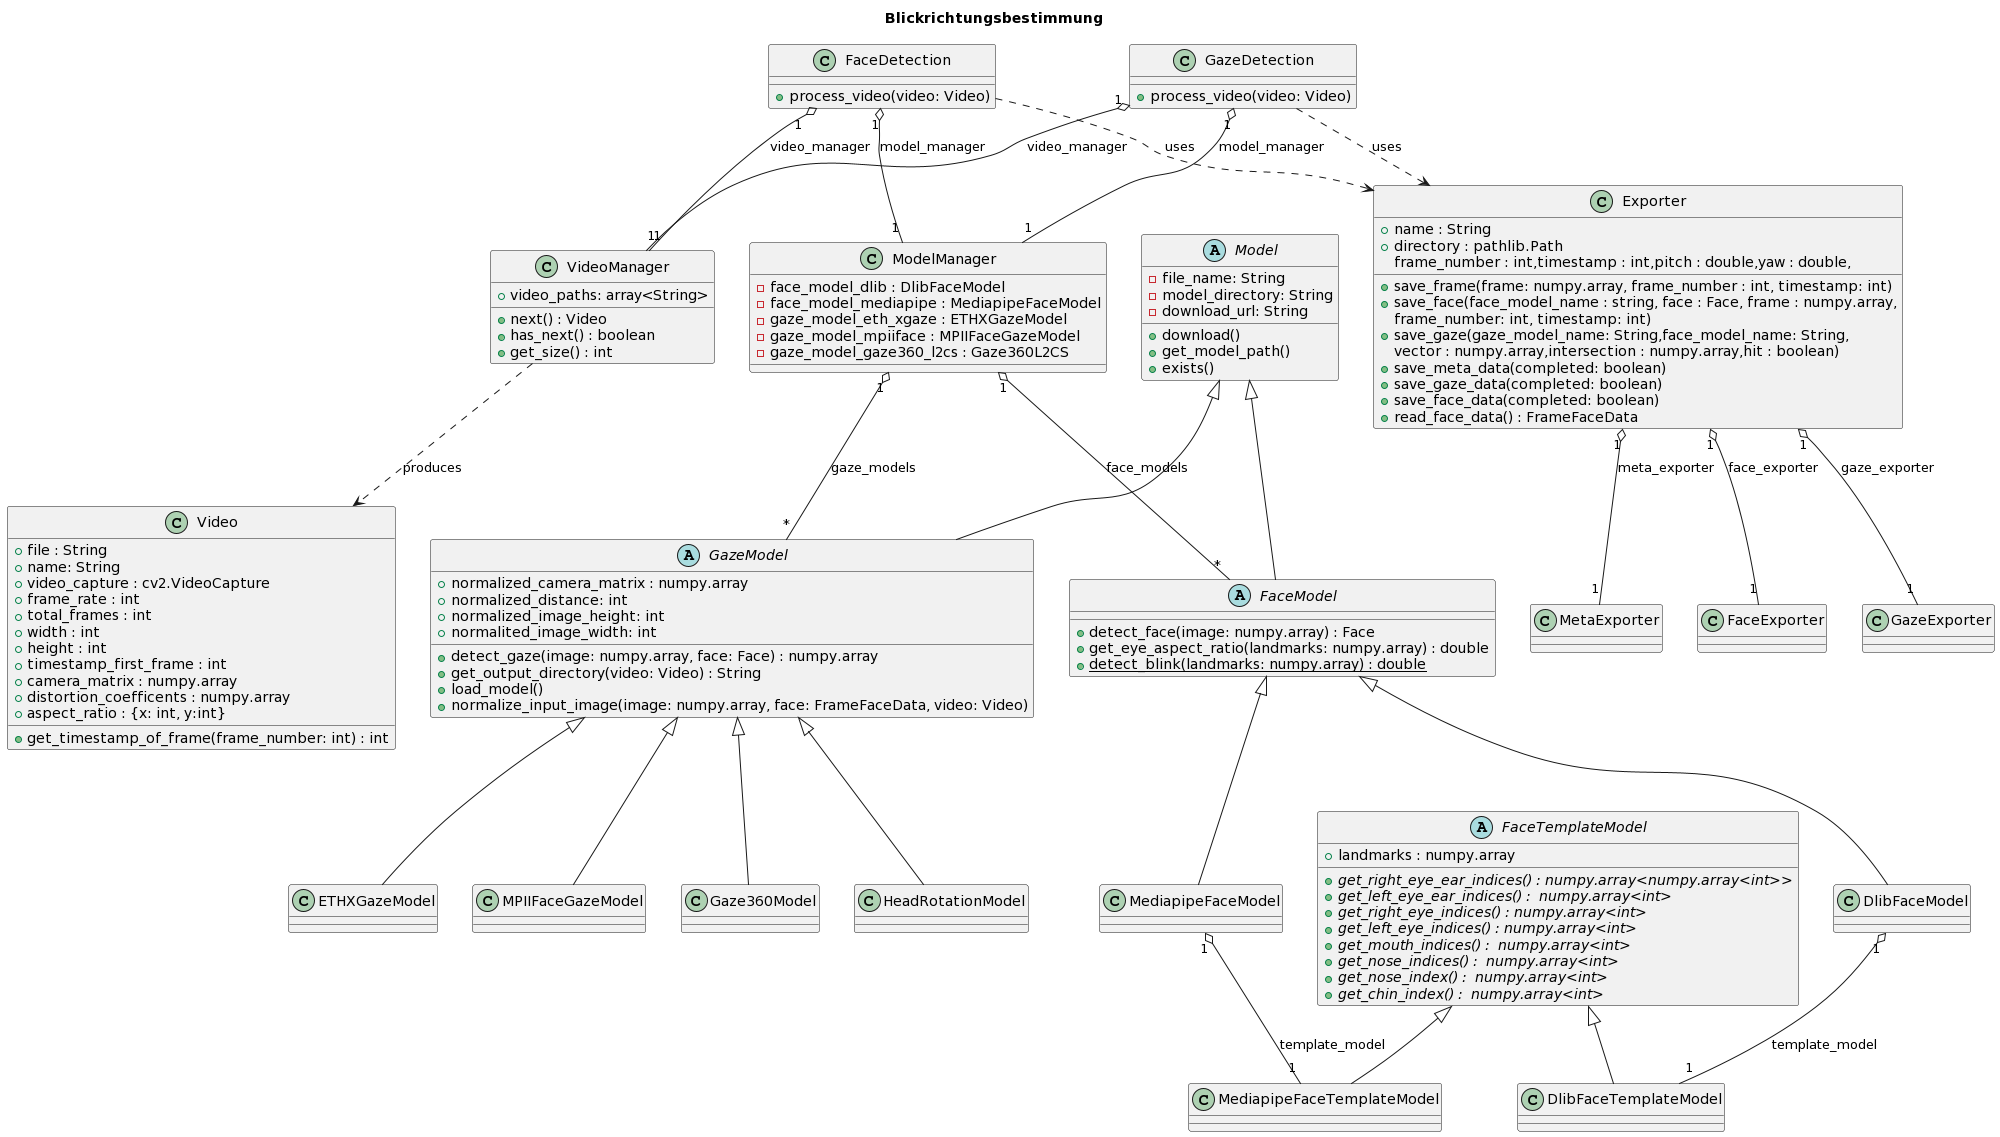
\includegraphics[width=\linewidth]{implementation/uml.png}
\caption{UML-Klassendiagramm\protect\footnote{Erstellt mit \url{https://www.planttext.com/} (Abgerufen am 09.11.2023)} des aktuellen Stands der Implementierung.}
\label{fig:implementation:uml}
\end{figure}

\section{Verarbeitung der Videos}\label{sec:implemenation:video}

Im ersten Schritt werden die Videos, die analysiert werden sollen, in die einzelne Frames der Videos zerlegt. Zudem werden weitere Details der Videos ermittelt, wie die Gesamtzahl der Frames eines Videos, die Anzahl der Frames pro Sekunde sowie die Höhe $\heightvideo$ und Breite $\widthvideo$ der Frames in Pixeln. Dafür wird die Python-Bibliothek von OpenCV\footnote{\url{https://github.com/opencv/opencv-python}  (24.10.2023)} \cite{paper:opencv} genutzt, welche Algorithmen für die Verarbeitung von Bildern und Videos bereitstellt. 

In der aktuellen Implementierung werden nur Videos im MP4-Format unterstützt, da bei der Aufnahme der Videos ausschließlich dieses Format verwendet wurde. OpenCV unterstützt jedoch eine Vielzahl von verschiedenen Videoformaten, wodurch bei Bedarf weitere Formate hinzugefügt werden können.

Anschließend werden die einzelnen Frames des Videos mithilfe von OpenCV iteriert. In der aktuellen Implementierung wird jedoch nur jeder dritte Frame verarbeitet, um den Aufwand während der Evaluation zu minimieren. Für jeden Frame $f$ wird dabei die Nummer $n$ sowie der Zeitpunkt des Frames $t$ in Millisekunden relativ zum Beginn des Videos bestimmt. Für die spätere Auswertung werden in diesem Schritt die ausgewählten Frames des Videos als Bild in einer separaten Datei gespeichert.  

\section{Erkennung und Verarbeitung von Gesichtsmerkmalen}\label{sec:implementation:face}

Für die in Kapitel \ref{sec:implemenation:video} ausgewählten Frames wird dann die Gesichtserkennung durchgeführt. Die Umsetzung von diesem Schritt wird in diesem Kapitel vorgestellt. Der generelle Ablauf der Gesichtserkennung ist in Abbildung \ref{fig:implementation:process:video} zu sehen.

\begin{figure}
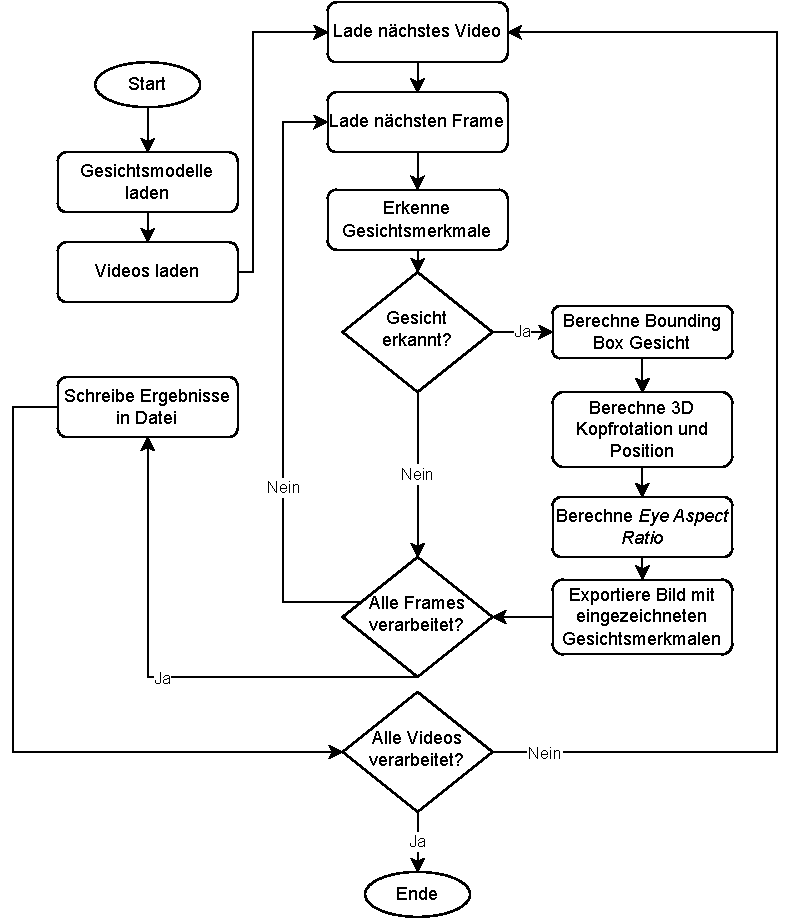
\includegraphics[width=0.5\linewidth]{implementation/process-face.pdf}
\caption{Ablauf der Gesichtserkennung.\protect\footnote{Erstellt mit \url{https://app.diagrams.net/} (Abgerufen am 09.11.2023)}}
\label{fig:implementation:process:video}
\end{figure}

\subsection{Identifizieren der Gesichtsmerkmale}\label{sec:implementation:face:landmarks}

Zunächst müssen die Gesichtsmerkmale der Radfahrenden identifiziert werden.
In Kapitel \ref{sec:concept:head} wurde festgelegt, dass zwei verschiedene Algorithmen zur Erkennung der Gesichtsmerkmale verwendet werden. Dabei handelt es sich um den \textit{ERT} Algorithmus \cite{paper:dlib} und die Gesichtserkennungspipeline von \mediapipe \cite{paper:mediapipe,paper:mediapipe:landmarks,paper:mediapipe:blazeface,paper:mediapipe:attention}.

Um den \textit{ERT} Algorithmus zu verwenden, wird die Implementierung des Algorithmus in der Open-Source Python Bibliothek\footnote{\url{https://pypi.org/project/dlib/} (Abgerufen am 21.08.2023)} von \dlib \cite{paper:dlib:main, paper:dlib} genutzt. Für die Erkennung von Gesichtsmerkmalen mit dem \mediapipe Framework wird das Python Package\footnote{\url{https://pypi.org/project/mediapipe/} (Abgerufen am 21.08.2023)} von \mediapipe verwendet.


Ziel ist nun eine Liste von einzelnen zweidimensionalen Gesichtspunkten $\landmark$ zu bestimmen, wobei $\indexlandmark$ den entsprechenden Index des Punktes in der Liste darstellt.
Das Erkennen der Gesichtsmerkmalen mit den beiden Methoden wird im Folgenden erläutert.

\subsubsection{MediaPipe}\label{sec:implementation:face:landmarks:mediapipe}

Für die Erkennung von Gesichtsmerkmalen mit \mediapipe wird die Klasse \textit{FaceMesh}\footnote{\url{https://github.com/google/mediapipe/blob/master/mediapipe/python/solutions/face_mesh.py} (Abgerufen am 21.11.2023)} des Frameworks verwendet.  Diese kombiniert den Schritt der Gesichtserkennung innerhalb des Bildes mit der Erkennung von insgesamt 468 Gesichtspunkten. Ein Beispiel für ein Bild mit erkannten Gesichtsmerkmalen ist in Abbildung \ref{fig:implementation:landmarks:mediapipe} zu sehen.

Die Klasse \textit{FaceMesh} kann über verschiedene Parameter konfiguriert werden. Zunächst kann festgelegt werden, ob das angezeigte Bild als einzelnes statisches Bild betrachtet werden soll oder ob das Bild Teil eines Videos ist und somit in Beziehung zu den vorhergehenden Bildern steht. Es wurde entschieden, das Bild einzeln zu betrachten. Dies wurde gemacht, da bei ersten Tests festgestellt wurde, dass sich ein Fehler bei der Gesichtserkennung sonst über mehrere Bilder erstreckt und immer nur stückweise korrigiert wird, um einen angenehmen Übergang beim Betrachten des Videos zu schaffen.
Darüber hinaus bietet \mediapipe mit dem Parameter \textit{refine\_landmarks} die Möglichkeit, die erkannten Punkte an markanten Stellen des Gesichts, zum Beispiel um das Auge und den Mund, weiter zu verfeinern \cite{paper:mediapipe:attention}. Dabei werden zusätzlich zehn weitere Gesichtspunkte zu den bereits erkannten hinzugefügt, welche die Iris der beiden Augen des Menschen darstellen. Es wurde sich dazu entschieden diese Verfeinerung der Gesichtspunkte durchzuführen. Die dabei zusätzlich erkannten Gesichtsmerkmale werden jedoch verworfen, da sie für die weitere Betrachtung der Gesichtserkennung ohne Bedeutung sind.
Weiterhin kann die erforderliche Zuversicht des Modells für die erfolgreiche Erkennung des Gesichts und der Gesichtsmerkmale konfiguriert werden. Diese wird als Wert zwischen 0 und 1 angegeben und ist standardmäßig auf 0,5 eingestellt. Bei Tests wurde jedoch festgestellt, dass die Standardzuversicht zu gering ist, da die Drehung des Kopfes des Radfahrenden häufig zu falsch erkannten Gesichtern geführt hat. Durch Ausprobieren wurde die erforderliche Mindestzuversicht des Modells für beide Erkennungen auf 0,8 festgelegt. Es ist jedoch anzumerken, dass keine Aussage darüber getroffen werden kann, welche Konfiguration für den Anwendungsfall in der PrioBike-App wirklich ideal ist, da die Qualität der Gesichtsmerkmalsbestimmung, wie bereits in Kapitel \ref{sec:concept:head} erwähnt, nur mit sehr großem Aufwand bewertet werden kann. Entweder man markiert für jedes Bild manuell die tatsächlichen Gesichtsmerkmale im Bild, um eine Ground Truth zu erstellen, was im zeitlichen Rahmen dieser Arbeit leider nicht umsetzbar war, oder ein Mensch klassifiziert die Qualität manuell durch das Betrachten der erkannten Gesichtsmerkmale jedes Mal neu, sobald man einen der Parameter angepasst hat, was im zeitlichen Rahmen dieser Arbeit ebenfalls nicht umsetzbar war.

Mit \mediapipe kann eine Liste von 468 einzelnen Gesichtsmerkmalen $\landmark$ in Form von dreidimensionalen Punkten, bestehend aus $\landmarkxnorm$, $\landmarkynorm$ und $\landmarkznorm$, ermittelt werden. $\landmarkxnorm$ gibt die normierte Position entlang der Breite des Bildes $\widthvideo$ an, $\landmarkynorm$ die normierte Position entlang der Höhe des Bildes $\heightvideo$. Die Koordinate $\landmarkznorm$ gibt einen normierten Tiefenwert für jeden Punkt an. Wie in Kapitel \ref{sec:concept:head:3d} beschrieben, soll aus den zweidimensionalen Bildkoordinaten eines Gesichtspunktes auf einen dreidimensionalen Gesichtspunkt relativ zur Kamera geschlossen werden. Mit dieser Methode liegen bereits dreidimensionale Punkte vor. Um jedoch eine bessere Vergleichbarkeit der beiden Methoden zur Bestimmung der Gesichtsmerkmale zu ermöglichen, soll die dreidimensionale Lage der Punkte auf die gleiche Weise bestimmt werden, weshalb die von \mediapipe bestimmte Tiefe der Punkte nicht weiter verwendet wird. Für mögliche zukünftige Experimente werden die Koordinaten jedoch gespeichert.

Für die in Kapitel \ref{sec:implementation:face:3d} beschriebene dreidimensionale Positionsbestimmung werden die Bildkoordinaten der Gesichtspunkte in Pixeln benötigt, weshalb die normierten Werte in Bildkoordinaten $\landmarkxbild$, $\landmarkybild$ umgerechnet werden.
 
\[
\landmarkxbild = \landmarkxnorm \cdot \widthvideo \qquad \landmarkybild = \landmarkynorm \cdot \heightvideo
\]

\subsubsection{dlib}

Um mit \dlib Gesichtspunkte zu bestimmen, muss zunächst im Bild ein Gesicht erkannt werden. Dafür wird der von \dlib Bibliothek bereitgestellte \textit{Face Detector} verwendet \cite{paper:dlib:face}. Die erkannten Gesichter liegen dann in Form einer Bounding Box vor. Anschließend wird mittels des von \dlib\footnote{\url{http://dlib.net/files/shape_predictor_68_face_landmarks.dat.bz2} (Abgerufen am 24.08.2023)} bereitgestellten \textit{Shape Predictors} 68 verschiedene Gesichtsmerkmale im Bild erkannt, welche in Form einer Liste von zweidimensionalen Bildkoordinaten $\landmarkxbild$ und $\landmarkybild$ vorliegen. Ein Beispiel für diese 68 erkannten Gesichtspunkte sind in Abbildung \ref{fig:implementation:landmarks:dlib} zu sehen.

Da die Koordinaten der Gesichtspunkte bei \mediapipe sowohl in normalisierter Form als auch in Bildkoordinaten vorliegen, wurden die Koordinaten $\landmarkxbild$ und $\landmarkybild$ aus Konsistenzgründen ebenfalls in die zweidimensionalen Koordinaten $\landmarkxnorm$, $\landmarkynorm$ umgewandelt. Wie bereits im Kapitel \ref{sec:implementation:face:landmarks:mediapipe} erläutert, wird die durch \mediapipe ermittelte Tiefe in Form der $\landmarkznorm$ Koordinate zwar nicht verwendet, aber dennoch gespeichert. \textit{Dlib} kann keine Auskunft über die Tiefe der Gesichtspunkte geben. Aus Konsistenzgründen wird aber ein Wert für $\landmarkznorm$ gespeichert werden. Dieser wurde für alle Gesichtspunkte auf 1 gesetzt. 

\[
\landmarkxnorm = \frac{\landmarkxbild}{\widthvideo} \qquad \landmarkynorm = \frac{\landmarkybild}{\heightvideo} \qquad \landmarkznorm = 1
\]


\begin{figure}[]
    \begin{subfigure}{0.425\textwidth}
        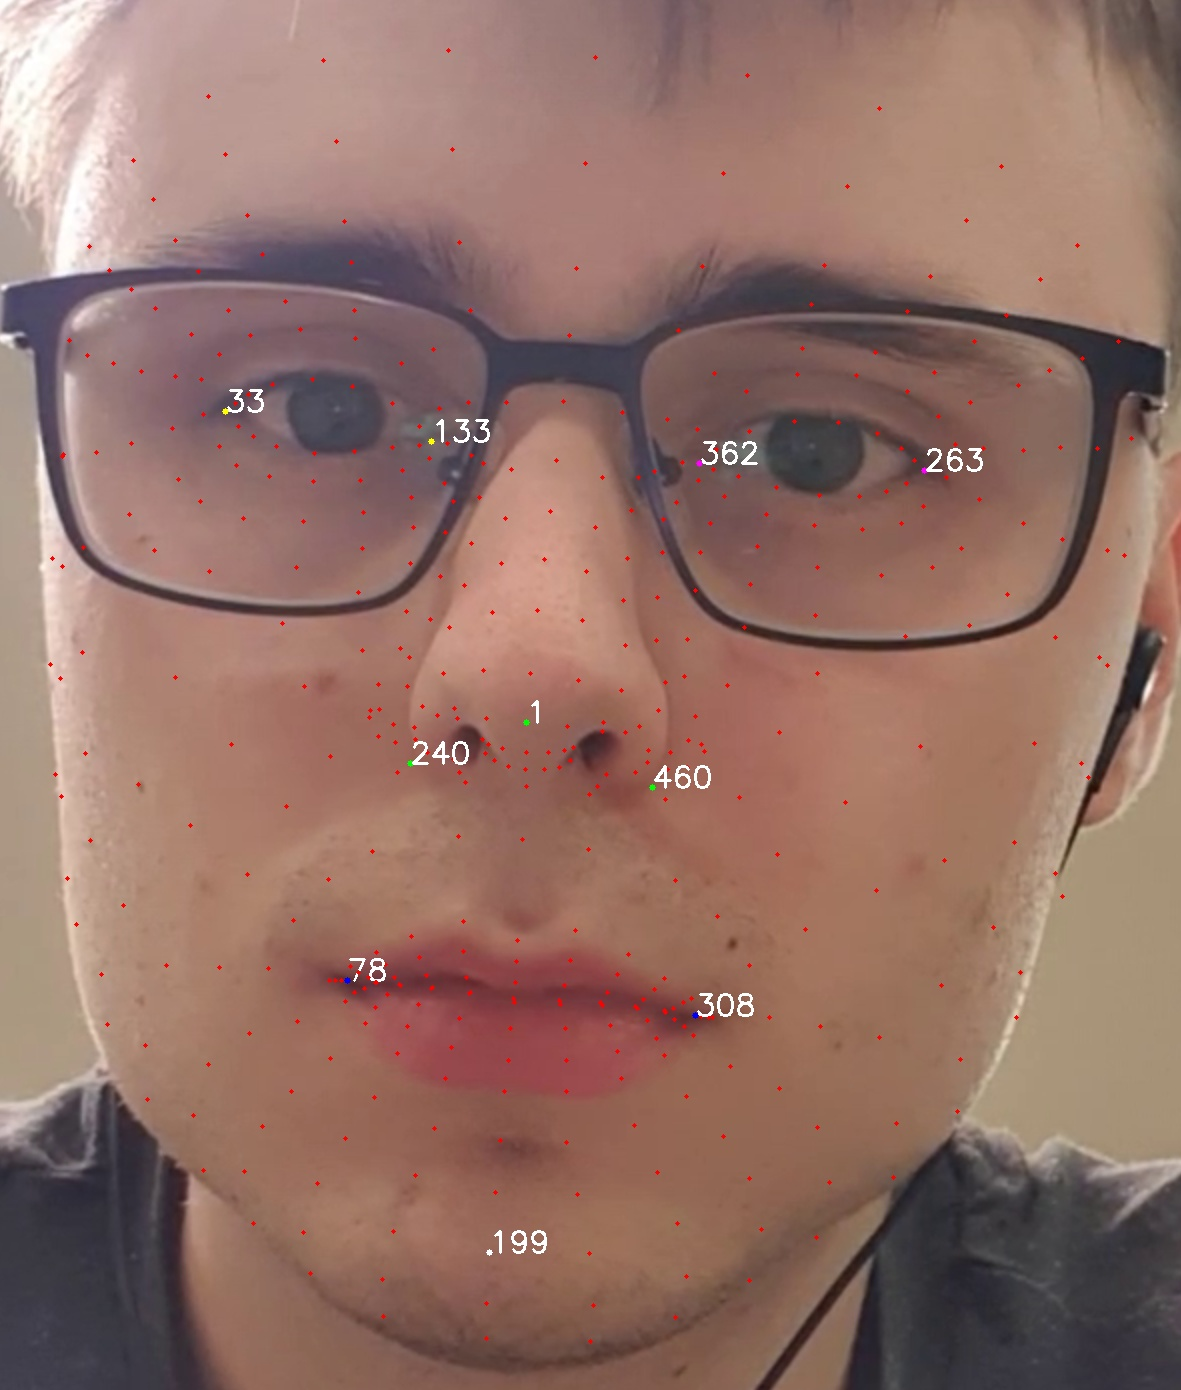
\includegraphics[width=\linewidth]{implementation/mediapipe.jpg}
        \caption{Beispiel von 468 Gesichtsmerkmalen mit \mediapipe}
        \label{fig:implementation:landmarks:mediapipe}
    \end{subfigure}%
    \hspace{0.5cm}
    \begin{subfigure}{0.475\textwidth}
        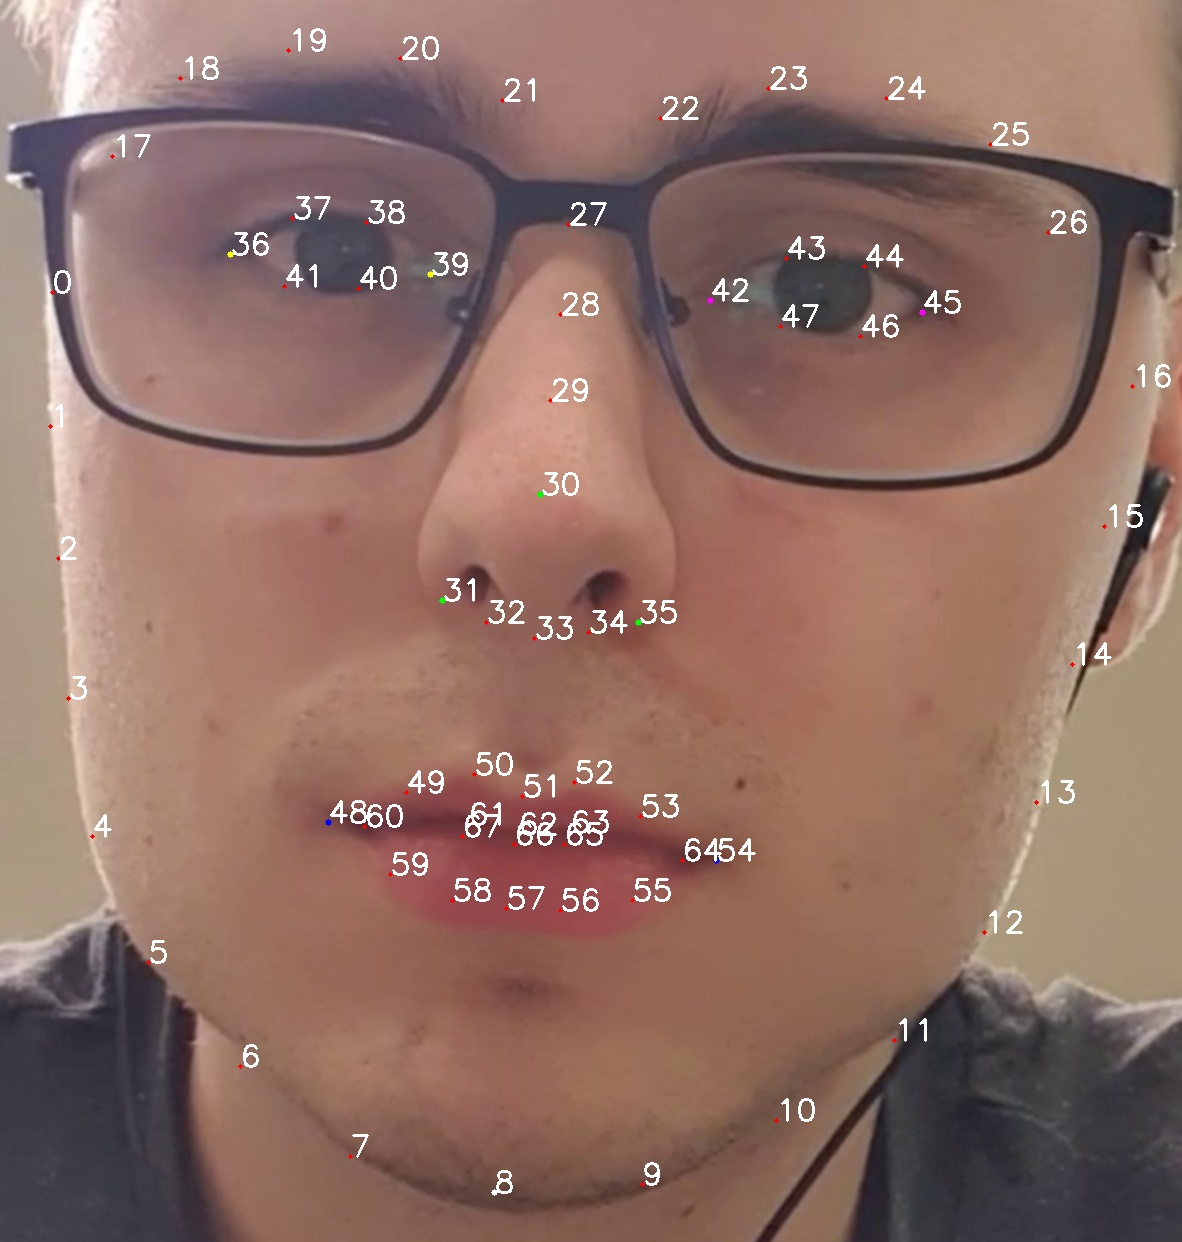
\includegraphics[width=\linewidth]{implementation/dlib.jpg}
        \caption{Beispiel von 68 Gesichtsmerkmalen mit der \dlib Bibliothek}
        \label{fig:implementation:landmarks:dlib}
    \end{subfigure}
    \caption{Beispiele für erkannte Gesichtsmerkmale mit \mediapipe und \dlib. Diese Gesichtsmerkmale sind anhand ihres Index $\indexlandmark$ beschriftet. In Abbildung \ref{fig:implementation:landmarks:mediapipe} sind aus Gründen der Übersichtlichkeit nur die wichtigsten Gesichtsmerkmale nummeriert.}
    \label{fig:implementation:landmarks}
\end{figure}

\subsection{Identifizieren von geschlossenen Augen}\label{sec:implementation:gaze:ear}

Aus den ermittelten zweidimensionalen Koordinaten $\landmarkxbild$ und $\landmarkybild$ eines Bildpunktes $\landmark$ wird nun das im Kapitel \ref{sec:concept:3d} beschriebene Verfahren zur Erkennung geschlossener Augen \cite{paper:ear} implementiert. Bei diesem Verfahren wird das \textit{Eye Aspect Ratio} ($EAR$) berechnet. Dazu werden sechs Punkte $P_1$ bis $P_6$ um das linke und rechte Auge benötigt. Die dafür verwendeten Gesichtsmerkmale $\landmark$ von \mediapipe und \dlib sind in Tabelle \ref{tab:implementation:ear} dargestellt.

\[
\ear_{\text{links/rechts}} = \frac{\|P_2 - P_6\| + \|P_3 - P_5\|}{2\|P_1 - P_4\|} \qquad \ear = \frac{\ear_{\text{links}} + \ear_{\text{rechts}}}{2}
\]

Anschließend muss ein Grenzwert $\earthreshold$ ermittelt werden. Ist der ermittelte $\ear$ Wert größer als $\earthreshold$, dann sind die Augen geöffnet. Wenn der Wert kleiner ist als $\earthreshold$, sind die Augen geschlossen. Dieser Grenzwert $\earthreshold$ wurde in der Evaluation für \dlib und \mediapipe bestimmt. Für \dlib beträgt der Wert 0,173 und für \mediapipe 0,159. Näheres dazu wird in Kapitel \ref{sec:evaluation:results:gaze:ear} erläutert.

\begin{table}[]
    \centering
    \begin{tabular}{c | c c | c c}
        \toprule
        & \multicolumn{2}{c|}{\textbf{dlib}} &\multicolumn{2}{c}{\textbf{MediaPipe}} \\
        \midrule
        \textbf{Punkt} & Linkes Auge & Rechtes Auge & Linkes Auge & Rechtes Auge \\
        \midrule
        $P_1$ & 42 & 36 & 362 & 33 \\
        $P_2$ & 43 & 37 & 385 & 160 \\
        $P_3$ & 44 & 38 & 387 & 158 \\
        $P_4$ & 45 & 39 & 263 & 133 \\
        $P_5$ & 46 & 40 & 373 & 153 \\
        $P_6$ & 47 & 41 & 380 & 144 \\
        \bottomrule
    \end{tabular}
    \caption{Verwendete Gesichtsmerkmale zur Bestimmung des $\ear$. Siehe Abbildung \ref{fig:implementation:landmarks}.}
    \label{tab:implementation:ear}
\end{table}

\subsection{Exportieren der Bilder mit erkannten Gesichtsmerkmalen}\label{sec:implementation:face:export:landmarks}

Wie in Kapitel \ref{sec:concept:head} beschrieben, soll die Gesichtserkennung in der Evaluation durch einen Menschen qualitativ beurteilt werden. Um diese Beurteilung zu ermöglichen, werden die zweidimensionalen Bildkoordinaten $\landmarkxbild$ und $\landmarkybild$ mittels der OpenCV-Bibliothek farblich markiert. Zusätzlich wird anhand dieser Punkte eine Bounding Box um das Gesicht berechnet, mit der das Bild auf das Gesicht zugeschnitten wird. Um die Beurteilung der Gesichtspunkte für einen Menschen zu erleichtern, werden markante Gesichtspunkte an Augen, Nase, Mundwinkel und Kinn farblich hervorgehoben. Die dafür verwendeten Gesichtsmerkmale sind in der Tabelle \ref{tab:implementation:used:landmarks} aufgeführt.
 
\begin{table}[]
    \centering
    \begin{tabular}{l c c }
    \toprule
        \textbf{Gesichtsmerkmal} & \textbf{dlib} & \textbf{MediaPipe} \\ \midrule
        Linkes Auge & 36, 39 & 33, 133 \\
        Rechtes Auge & 42, 45 & 263, 362 \\
        Mund & 48, 54 & 78, 308 \\
        Nase & 31, 35& 240, 460\\
        Nasenspitze & 30 & 1 \\
        Kinn & 8 & 199\\
        \bottomrule
    \end{tabular}
    \caption{Farblich hervorgehobene Gesichtspunkte für die Evaluation der erkannten Gesichtsmerkmale.}
    \label{tab:implementation:used:landmarks}
\end{table}

\subsection{Dreidimensionale Kopfrotation bestimmen}\label{sec:implementation:face:3d}

Wie in Kapitel \ref{sec:concept:head:3d} beschrieben, wird für die weitere Bestimmung der Blickrichtung die dreidimensionale Position des Kopfes relativ zur Kamera benötigt. Ein Ansatz hierfür wurde ebenfalls in Kapitel \ref{sec:concept:head:3d} beschrieben \cite{paper:eth-xgaze, paper:mpiigaze}. Für diesen Ansatz wird ein dreidimensionales, statisch ausgerichtetes Modell des Kopfes mit der gleichen Anzahl von Punkten benötigt, wie Gesichtspunkte erkannt werden - also ein dreidimensionales Modell des Kopfes mit 68 Punkten für die Erkennung mit \dlib und ein Modell mit 468 Punkten für die Erkennung mit \mediapipe. Die verwendeten Modelle stammen aus der \textit{pt-gaze} Python Bibliothek\footnote{\url{https://pypi.org/project/ptgaze/} (Abgerufen am 25.08.2023). 68 Gesichtsmerkmale: \url{https://github.com/hysts/pytorch_mpiigaze_demo/blob/master/ptgaze/common/face_model_68.py} (Abgerufen am 01.11.2023), 468 Gesichtsmerkmale: \url{https://github.com/hysts/pytorch_mpiigaze_demo/blob/master/ptgaze/common/face_model_mediapipe.py} (Abgerufen am 01.11.2023)}, welche die Funktionsweise von verschiedenen neuronalen Netzwerken zur Bestimmung von Blickrichtungen demonstriert. Eine Darstellung dieser Kopfmodelle ist in Abbildung \ref{fig:implementation:templates} zu sehen.

\begin{figure}[]
    \begin{subfigure}{0.5\textwidth}
        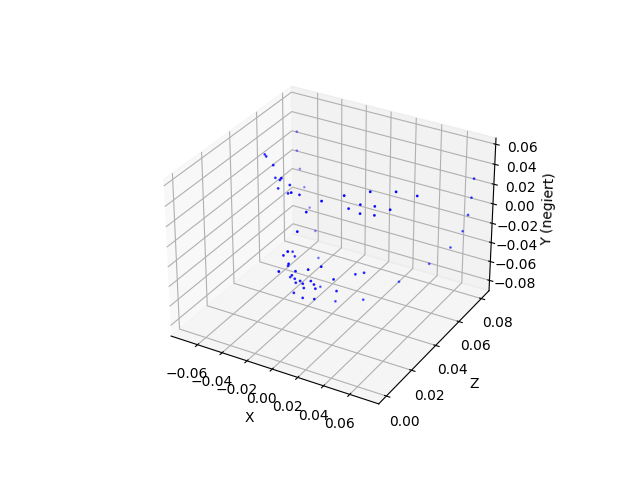
\includegraphics[width=\linewidth]{implementation/68_face_template_model.png}
        \caption{3D Gesichtsmodell bestehend aus 68 Punkten}
        \label{fig:implement:templates:dlib}
    \end{subfigure}%
    \begin{subfigure}{0.5\textwidth}
        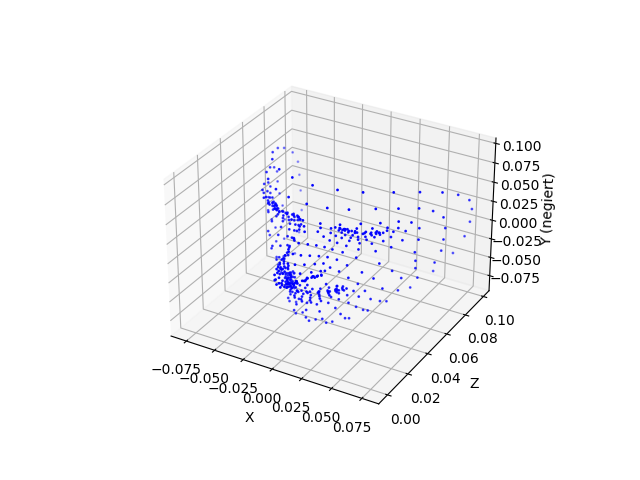
\includegraphics[width=\linewidth]{implementation/468_face_template_model.png}
        \caption{3D Gesichtsmodell bestehend aus 468 Punkten}
        \label{fig:implement:templates:mediapipe}
    \end{subfigure}
    \caption{Verwendete dreidimensionale Modelle des Kopfes mit 68 Punkten (Abbildung \ref{fig:implement:templates:dlib}) und 468 Punkten (Abbildung \ref{fig:implement:templates:mediapipe}). Zur Darstellung wurde jeweils die y-Achse invertiert.}
    \label{fig:implementation:templates}
\end{figure}

Zur Bestimmung der dreidimensionalen Position der Punkte bietet OpenCV die \textit{solvePnP} Funktion\footnote{\url{https://docs.opencv.org/4.x/d5/d1f/calib3d_solvePnP.html} (Abgerufen am 25.09.2023)} an. Mit dieser können mittels der intrinsischen Parameter der Kamera, der Liste der erkannten zweidimensionalen Gesichtspunkte und der Liste der dreidimensionalen Punkte des Modells ein Rotationsvektor $\rotationvector$ und ein Translationsvektor $\translationvector$ berechnet werden. Diese geben an, wie das dreidimensionale Modell des Kopfes gedreht und verschoben werden muss, um der dargestellten zweidimensionalen Pose zu entsprechen.

Das dreidimensionale Koordinatensystem kann dabei wie folgt beschrieben werden:

\begin{itemize}
    \item Die Kamera befindet sich im Koordinatenursprung.
    \item Die x-Achse zeigt relativ zur Kamera nach rechts und gibt die relative Position in der Breite des Bildes an.
    \item Die y-Achse zeigt relativ zur Kamera nach unten und gibt die relative Position in der Höhe des Bildes an. 
    \item Die z-Achse zeigt relativ zur Kamera nach vorn und gibt die Tiefe des Bildpunktes zur Kamera an.
\end{itemize}

Bevor das Problem gelöst werden kann, müssen die intrinischen Parameter der Kamera bestimmt werden. Dazu gehören eine Kameramatrix $\cameramatrix$ und die Verzerrungskoeffizienten der Smartphone-Kamera, mit der das Video aufgenommen wurde. Um diese exakt zu bestimmen, muss die Kamera kalibriert werden. OpenCV bietet hierfür die Funktion \textit{calibrateCamera}\footnote{\url{https://docs.opencv.org/3.4/dc/dbb/tutorial_py_calibration.html} (Abgerufen am 20.11.2023)}, mit der diese Parameter bestimmt werden können. Dazu ist jedoch ein spezieller Kalibrierungsprozess erforderlich, bei dem zum Beispiel Bilder von einem Schachbrett mit einem bestimmten Abstand der Kamera zu diesem Schachbrett aufgenommen werden. Da dieser Kalibrierungsprozess für jede Kamera durchgeführt werden müsste, ist er ungeeignet für den Anwendungsfall der PrioBike-App. Daher wurden diese Parameter geschätzt. Es ist zu beachten, dass dies zu ungenaueren Ergebnissen führt, als wenn diese Parameter exakt bestimmt würden. Zunächst wird für jedes aufgenommene Video eine Kameramatrix $\cameramatrix$ erstellt. Dazu wird die Brennweite entlang der Bildbreite sowie der Bildlänge als Bildgröße in Pixeln angenommen. Das optische Zentrum des Bildes wird in der Bildmitte angenommen.

\[
c_w = \frac{\widthvideo}{2} \qquad
c_h = \frac{\heightvideo}{2} \qquad  
\cameramatrix = \begin{pmatrix}
\widthvideo & 0 & c_w \\
0 & \heightvideo & c_h \\
0 & 0 & 1\\
\end{pmatrix}
\]

Das Bild einer Kamera kann durch radiale und tangentiale Verzerrungen beeinflusst werden. Die radiale Verzerrung bewirkt, dass eine gerade Linie in einem Bild gekrümmt wird. Die tangentiale Verzerrung führt dazu, dass Teile des Bilder näher an der Kamera erscheinen, als sie eigentlich sind. Diese Verzerrung des Bildes kann angegeben werden mittels der Verzerrungskoeffizienten $k_1$, $k_2$, und $k_3$, welche die radiale Verzerrung beschreiben, sowie mit $p_1$ und $p_2$, welche die tangentiale Verzerrung beschreiben \footnote{Siehe \url{https://docs.opencv.org/4.x/dc/dbb/tutorial_py_calibration.html} (Abgerufen am 02.11.2023)}. Kennt man diese Koeffizienten, kann man die Verzerrung des Bildes korrigieren. Im Anwendungsfall der PrioBike-App ist jedoch nicht mit größeren Verzerrungen der Bilder durch die Innenkamera des Smartphones zu rechnen. Daher werden diese Koeffizienten als 0 angenommen.

\[
\text{Verzerrungskoeffizienten} = (k_1, k_2, p_1, p_2, k_3) = (0, 0, 0, 0, 0)
\]

Nachdem diese Parameter geschätzt wurden, kann die Funktion ausgeführt werden.
Wie bereits erwähnt, liefert die Funktion als Ergebnis einen Rotationsvektor $\rotationvector$ und einen Translationsvektor $\translationvector$. Aus $\rotationvector$ wird im nächsten Schritt eine Rotationsmatrix $\rotationmatrix$ berechnet:

\[
\rotationvector = \begin{pmatrix}
    r_x \\ r_y \\ r_z
\end{pmatrix} \\
\]

\[
\theta = \|\vec{r}\| \qquad
\omega =  1- \cos \theta \qquad
\alpha = \frac{r_x}{\theta} \qquad
\beta = \frac{r_y}{\theta} \qquad
\gamma = \frac{r_z}{\theta}
\]

\[
\rotationmatrix = \begin{pmatrix}
    \alpha^2\cdot\omega + \cos \theta & \alpha\cdot\beta\cdot\omega - \gamma \cdot\sin\theta & \alpha\cdot\gamma\cdot\omega + \beta\cdot\sin\theta \\
    \alpha\cdot\beta\cdot\omega + \gamma \cdot \sin \theta & \beta^2 \cdot\omega+\cos\theta & \beta\cdot\gamma\cdot\omega-\alpha\cdot\theta \\
    \alpha\cdot\gamma\cdot\omega - \beta \cdot \sin\theta & \beta\cdot\gamma\cdot\omega + \alpha\cdot\sin\theta & \gamma^2\cdot\omega+\cos\theta \\
\end{pmatrix}
\]

Mittels der bestimmten Rotationsmatrix $\rotationmatrix$ und dem Translationsvektor $\translationvector$  können die Punkte des Kopfmodells $F_i$ (wobei $i$ der Index des entsprechenden zweidimensionalen Gesichtspunkt $\landmark$ ist) nun so rotiert und verschoben werden, dass sie der dreidimensionalen Position des dargestellten Gesichts entsprechen. Somit erhält man die dreidimensionale Position bestehend aus $\landmarkxmodel$, $\landmarkymodel$, $\landmarkzmodel$ für jeden Gesichtspunkt $L_i$.

\[
\begin{pmatrix}
   \landmarkxmodel \\ \landmarkymodel \\ \landmarkzmodel \\ 
\end{pmatrix} = F_i \cdot \rotationmatrix^T + \translationvector
\]

Anhand der dreidimensionalen Position der Gesichtspunkte kann nun das Zentrum des Kopfes $\centerface$ im dreidimensionalen Raum berechnet werden. Dieser wird definiert als das Zentrum der äußersten Punkte der Augen sowie den äußersten Punkte der Nase. Die dafür verwendeten Gesichtspunkte sind in der Tabelle  \ref{tab:implementation:used:landmarks} zu sehen.
Aus diesem Punkt $\centerface$ kann nun der Abstand des Kopfes zur Kamera im Koordinatenursprung, im folgenden $\distancefacecamera$ genannt, berechnet werden. Die Distanz $\distancefacecamera$ entspricht der Länge des Vektors vom Koordinatenursprung zu Punkt $\centerface$.

\subsection{Persistenz der Ergebnisse}

Die Ergebnisse der Gesichtserkennung eines Videos werden für jedes verwendete Gesichtsmodell in einer separaten Datei gespeichert. Die Datei ist folgendermaßen aufgebaut: In der ersten Zeile steht ein Wahrheitswert, der angibt, ob die Gesichtserkennung für das entsprechende Video vollständig abgeschlossen wurde oder nicht. Anschließend wird für jedes ausgewählte Frame $f$, in dem ein Gesicht erkannt werden konnte, ein Eintrag in die Datei eingefügt. Zu einem Eintrag gehören:

\begin{itemize}
    \item Nummer des Frames $f$ ($n$)
    \item Zeitpunkt des Frames $f$ in Millisekunden ($t$)
    \item Distanz $\distancefacecamera$
    \item Rotationsvektor $\vec{r}$
    \item Kopfzentrum $C$
    \item Translationsvektor $\translationvector$ 
    \item $EAR$
    \item Auflistung erkannter Gesichtspunkte $\landmark$
    \begin{itemize}
        \item Index $\indexlandmark$
        \item $\landmarkxmodel$
        \item $\landmarkymodel$
        \item $\landmarkzmodel$
        \item $\landmarkxnorm$
        \item $\landmarkynorm$
        \item $\landmarkznorm$
        \item $\landmarkxbild$
        \item $\landmarkybild$
    \end{itemize}
\end{itemize}

Die einzelnen Einträge sind durch eine Leerzeile getrennt. Wenn für ein Bild kein Gesicht erkannt wurde, wird in der Datei kein Eintrag erstellt. Ein Beispiel für eine solche Datei ist in Abbildung \ref{code:implementation:face:output} dargestellt.

\begin{figure}
    \centering
   \begin{lstlisting}[language=Java]
true // Video wurde vollstaendig verarbeitet

0 // Nummer des Frames 
0 // Zeitpuntk des Frames
0.2617788121569677 // Distanz zwischen Gesicht und Kamera
-0.04532,-0.01643,0.08828 // Rotationsvektor des Gesichts
-0.01548,-0.02905,0.2597 // Kopfzentrum
-0.0165,-0.0125,0.22876 // Translationsvektor des Gesichts
0.4318541506079564 // EAR
0,-0.08664,-0.04335,0.31008,0.2056,0.4109,1,222,789 // Gesichtspunkt mit Index 0
1,-0.08752,-0.02475,0.30845,0.2046,0.4464,1,221,857 // Gesichtspunkt mit Index 1
... // Face Landmarks mit Index 2 bis 66
67,-0.0278,0.02461,0.24632,0.3944,0.5521,1,426,1060 // Gesichtspunkt mit Index 67

3
99
0.2608503005208114
-0.04663,-0.00485,0.08932
-0.01503,-0.02871,0.25883
-0.01642,-0.01222,0.22787
0.5655616094861263
0,-0.0856,-0.04296,0.31005,0.2074,0.4156,1,224,798
1,-0.08651,-0.02437,0.3084,0.2056,0.4495,1,222,863
...
\end{lstlisting}
    \caption{Ausschnitt aus der Ergebnisdatei der Gesichtserkennung mit \dlib.}
    \label{code:implementation:face:output}
\end{figure}

\section{Blickrichtungsbestimmung}\label{sec:implementation:gaze}

Nachdem die Gesichtserkennung durchgeführt wurde, wird aufbauend auf den Ergebnissen der Gesichtserkennung die Blickrichtungsbestimmung durchgeführt. Hierfür wurden zwei unterschiedliche Konzepte erarbeitet. Zum einen soll die Blickrichtung mithilfe von Convolutional Neural Networks aus dem Gesicht des Radfahrers bestimmt werden, wie in Kapitel \ref{sec:concept:3d} erläutert wird. Das zweite Konzept verwendet die bei der Gesichtserkennung ermittelte Kopfdrehung als Blickrichtung, wie in Kapitel \ref{sec:concept:head} beschrieben wird. Die Implementierung der beiden Methoden zur Bestimmung der Blickrichtung und die Interpretation der Ergebnisse werden im Folgenden vorgestellt.

\subsection{Blickrichtungsbestimmung mit Convolutional Neural Networks}\label{sec:implementation:gaze:vector:models}

Im Folgenden wird die Blickrichtungsbestimmung mittels Convolutional Neural Networks beschrieben. Dazu wird zunächst die Implementierung der Modelle erläutert. Anschließend wird die Implementierung des von Cheng et al. vorgestellten Verfahrens zur Bildnormalisierung \cite{paper:basics:survey} beschrieben. Abschließend wird gezeigt, wie die Ergebnisse der Convolutional Neural Networks verwendet werden können, um einen dreidimensionalen Blickrichtungsvektor $\gazevector$ zu bestimmen.


\subsubsection{Implementierung der Convolutional Neural Networks}

Wie in Kapitel \ref{sec:concept:3d} beschrieben, wurden die Datensätze \textit{ETH-XGaze} \cite{paper:eth-xgaze}, \textit{Gaze360} \cite{paper:gaze360} und \textit{MPIIFaceGaze} \cite{paper:mpiifacegaze} ausgewählt, die als Grundlage für je ein \cnn dienen sollen. Für die generelle Implementierung der Modelle wird die \textit{PyTorch} Python Bibliothek\footnote{\url{https://pytorch.org/} (Abgerufen am 29.11.2023)} verwendet.

Für die Datensätze \ethg und \mpii stellt die \textit{pt-gaze}\footnote{\url{https://pypi.org/project/ptgaze/} (Abgerufen am 02.12.2023), \url{https://github.com/hysts/pytorch_mpiigaze_demo/tree/master} (Abgerufen am 02.12.2023)} Python Bibliothek jeweils eine Implementierung eines Convolutional Neural Networks zur Verfügung, die in dieser Arbeit verwendet werden. 

Die Implementierung des Modells, das den \ethg Datensatz verwendet, wird mit der \textit{PyTorch Image Models}\footnote{\url{https://pypi.org/project/timm/} (Abgerufen am 02.12.2023)} Python Bibliothek realisiert und beruht auf einer ResNet-18 Architektur. Zusätzlich werden die vortrainierten Gewichtungen des Modells\footnote{\url{https://github.com/hysts/pytorch_mpiigaze_demo/releases/download/v0.2.2/eth-xgaze_resnet18.pth} (Abgerufen am 25.08.2023)} durch die \textit{pt-gaze} Bibliothek bereitgestellt. 

Die Implementierung des Modells, das auf dem \mpii Datensatz beruht, kann in der \textit{pt-gaze} Bibliothek auf verschiedene Arten und Weisen konfiguriert werden. Im Rahmen dieser Arbeit wurde die Implementation des Modells\footnote{\url{https://github.com/hysts/pytorch_mpiigaze_demo/blob/master/ptgaze/models/mpiifacegaze/resnet_simple.py} (Abgerufen am 03.12.2023), Backbone: \url{https://github.com/hysts/pytorch_mpiigaze_demo/blob/master/ptgaze/models/mpiifacegaze/backbones/resnet_simple.py} (Abgerufen am 03.12.2023)} so angepasst, dass sie der Standardkonfiguration\footnote{\url{https://github.com/hysts/pytorch_mpiigaze_demo/blob/master/ptgaze/data/configs/mpiifacegaze.yaml} (Abgerufen am 03.12.2023)} der Bibliothek entspricht. Weiter musste eine Anpassungen an der Implementierung vorgenommen werden, da durch eine unterschiedliche Version des \textit{PyTorch torchvision} Python Packages ein Fehler aufgetreten ist. Speziell wird in der \textit{pt-gaze} Bibliothek das \textit{model\_urls} Attribut von \textit{torchvision.models.resnet} verwendet, um die vortrainierten Gewichtungen einer ResNet-18 Architektur zu laden. Dieses Attribut wird in der Version, die in dieser Arbeit genutzt wird\footnote{Version 0.15.2}, nicht mehr unterstützt. Daher wurde die entsprechende URL\footnote{Gemeint ist \url{https://download.pytorch.org/models/resnet18-f37072fd.pth} (Abgerufen am 03.12.2023)} manuell eingefügt. Auch für die Anwendung dieses Modells werden die vortrainierten Gewichtungen\footnote{\url{https://github.com/hysts/pytorch_mpiigaze_demo/releases/download/v0.1.0/mpiifacegaze_resnet_simple.pth} (Abgerufen am 25.08.2023)} der \textit{pt-gaze} Bibliothek verwendet. 

Für den \textit{Gaze360}-Datensatz wird die Implementierung von Abdelrahman et al. \textit{L2CS-net} \cite{paper:l2csnet} verwendet. Die Implementierung wurde in Kapitel \ref{sec:related:gaze:appearance:l2cs} vorgestellt und ist öffentlich zugänglich\footnote{\url{https://github.com/Ahmednull/L2CS-Net} (Abgerufen am 29.11.2023) verwendet. Die Implementierung des von Abdelrahman et al. vorgestellten Convolutional Neural Networks ist unter folgender URL zu finden: \url{https://github.com/Ahmednull/L2CS-Net/blob/main/l2cs/model.py} (Abgerufen am 29.11.2023)}. Auch Abdelrahman et al. stellen vortrainierte Gewichtungen\footnote{\url{https://drive.google.com/uc?id=18S956r4jnHtSeT8z8t3z8AoJZjVnNqPJ&export=download} (Abgerufen am 25.08.2023)} zur Verfügung, die in dieser Arbeit verwendet werden. Es ist jedoch aufgefallen, dass in der Implementierung von Abdelrahman et al. die Bedeutung der Pitch- und Yaw-Winkel\footnote{Siehe \url{https://github.com/Ahmednull/L2CS-Net/blob/a4d8f7fa5436a2b2b9f088471623b552a85811bd/l2cs/vis.py#L13C5-L14C39} (Abgerufen am 03.12.2023)} von der Definition in Kapitel \ref{sec:basics:eye} abweicht. Die entsprechenden Ergebnisse des Modells werden daher im Rahmen dieser Arbeit vertauscht.

Im Folgenden werden die Convolutional Neural Networks nach dem Datensatz benannt, mit dem sie trainiert wurden.

\subsubsection{Normalisierung}

Bevor die erkannten Gesichter der Radfahrenden mit den Convolutional Neural Networks verarbeitet werden können, müssen sie (wie in Kapitel \ref{sec:concept:3d}) beschrieben normalisiert werden. Dazu muss eine Projektionsmatrix $\projectionmatrix$ bestimmt werden. Für die Berechnung dieser Matrix werden folgende Daten benötigt:

\begin{itemize}
    \item die Rotationsmatrix $\rotationmatrix$, die aus dem bei der Gesichtserkennung gespeicherten Rotationsvektor $\rotationvector$ berechnet werden kann,
    \item ein Referenzpunkt im Gesicht der abgebildeten Person, um den die Kamera entlang der Längsachse gedreht wird (Zentrum des Kopfes $\centerface$),
    \item der Vektor $\vec{c}$, der vom Koordinatenursprung (Kamera) zum Zentrum des Kopfes $\centerface$ zeigt,
    \item die geschätzte Kameramatrix $\cameramatrix$ der Innenkamera des Smartphones,
    \item eine normalisierte Distanz $\hat{d}$, die den Abstand der virtuellen Kamera zum dargestellten Gesicht beschreibt,
    \item eine Skalierungsmatrix $\scalematrix$ zur Berechnung des virtuellen Abstands der Kamera zum Gesicht,
    \item die Größe des normalisierten Bildes in Pixeln,
    \item eine normalisierte Kameramatrix $\normcameramatrix$, die die virtuelle Kamera nach der Normalisierung beschreibt.
\end{itemize}

Die verwendeten normalisierten Kameramatrizen $\normcameramatrix$, Distanzen $\hat{d}$ und Bildgrößen für die Eingabebilder der einzelnen Modelle sind in Tabelle \ref{tab:implementation:gaze:camera:configs} aufgeführt.

\begin{table}[]
    \centering
    \begin{tabular}{l c c c}
    \toprule
        \textbf{Modell} & \makecell{\textbf{Normalisierte}\\ \textbf{Kameramatrix $\normcameramatrix$}}  & \textbf{Bildgröße} & \makecell{\textbf{Normalisierte}\\ \textbf{Distanz $\hat{d}$}}  \\ 
        \midrule
        ETH-XGaze\footnote{Die verwendete normalisierte Kameramatrix und Distanz stammen aus der \textit{pt-gaze} Bibliothek. Die Parameter sind unter folgender URL zu finden: \url{https://github.com/hysts/pytorch_mpiigaze_demo/blob/master/ptgaze/data/normalized_camera_params/eth-xgaze.yaml} (Abgerufen am 29.11.2023)} & $\begin{pmatrix}960 & 0 & 112 \\0 & 960 & 112 \\ 0 & 0 & 1 \end{pmatrix}$ & $224 \times 224$ & 0,6 \\
        MPIIFaceGaze\footnote{Die verwendete normalisierte Kameramatrix und Distanz stammen aus der \textit{pt-gaze} Bibliothek. Die Parameter sind unter folgender URL zu finden: \url{https://github.com/hysts/pytorch_mpiigaze_demo/blob/master/ptgaze/data/normalized_camera_params/mpiifacegaze.yaml} (Abgerufen am 29.11.2023)} & $\begin{pmatrix}1600 & 0 & 112 \\0 & 1600 & 112 \\ 0 & 0 & 1 \end{pmatrix}$ & $224 \times 224$ & 1\\
        Gaze360\footnote{Es werden die gleichen Parameter wie für \textit{ETH-XGaze} verwendet.} & $\begin{pmatrix}960 & 0 & 112 \\0 & 960 & 112 \\ 0 & 0 & 1 \end{pmatrix}$ & $224 \times 224$ & 0,6 \\
        \bottomrule
        
    \end{tabular}
    \caption{Darstellung der verwendeten Normalisierungsmatrizen, normalisierte Bildgröße und normalisierte Distanz $\hat{d}$, die für die einzelnen Datensätze, auf denen die Modelle basieren, verwendet wurden.}
    \label{tab:implementation:gaze:camera:configs}
\end{table}

Die Projektionsmatrix $\projectionmatrix$ kann dann wie folgt berechnet werden:

\[
\rotationmatrix = \begin{pmatrix}
    r_{11} & r_{12} & r_{13} \\
    r_{21} & r_{22} & r_{23} \\
    r_{31} & r_{32} & r_{33}
\end{pmatrix} \qquad R_x = \begin{pmatrix}
r_{11} \\
r_{21} \\
r_{31} 
\end{pmatrix} \qquad \scalematrix = \begin{pmatrix}
    1 & 0 & 0 \\
    0 & 1 & 0 \\
    0 & 0 & \frac{\hat{d}}{\distancefacecamera}
\end{pmatrix}
\]

\[
z_{\text{axis}} = \frac{\vec{c}}{\|\vec{c}\|} \qquad
y' = z_{\text{axis}} \times R_x \qquad
y_{\text{axis}} = \frac{y'}{\|y'\|} \qquad
x' = y_{\text{axis}} \times z_{\text{axis}} \qquad
x_{\text{axis}} = \frac{x'}{\|x'\|}
\]

\[
R_{\text{Normalisierung}} = \begin{pmatrix}
    x_{\text{axis},1} & x_{\text{axis},2} & x_{\text{axis},3} \\
    y_{\text{axis},1} & y_{\text{axis},2} & y_{\text{axis},3} \\
    z_{\text{axis},1} & z_{\text{axis},2} & z_{\text{axis},3}
\end{pmatrix}
\]

\[
T = \scalematrix \cdot R_{\text{Normalisierung}}
\]

\[
\projectionmatrix = \normcameramatrix \cdot T \cdot \cameramatrix^{-1}
\]

Diese Projektionsmatrix $\projectionmatrix$ kann dann für die Normalisierung des Bildes verwendet werden. Dazu wird die Funktion \textit{warpPerspective}\footnote{\url{https://docs.opencv.org/3.4/da/d54/group__imgproc__transform.html#gaf73673a7e8e18ec6963e3774e6a94b87} (Abgerufen am 29.11.2023)} von OpenCV verwendet. Mit dieser kann ein Bild mit gegebener Projektionsmatrix und normalisierter Bildgröße perspektivisch transformiert werden.

\subsubsection{Bestimmen der Blickrichtung}

Die normalisierten Bilder werden im Anschluss in die Convolutional Neural Networks geladen. Alle drei Modelle berechnen aus dem normalisierten Bild einen Pitch- und Yaw-Winkel, der die Blickrichtung der dargestellten normalisierten Person beschreibt. Diese beiden Winkel können wie folgt in den normalisierten Blickrichtungsvektor $\vec{g'}$ umgerechnet werden:

\[
 \vec{g'} = \begin{pmatrix}
     \cos(\text{pitch}) \cdot \sin(\text{yaw}) \\
    \sin(\text{pitch}) \\
     \cos(\text{pitch}) \cdot \cos(\text{yaw}) \\
 \end{pmatrix}
\]

Anhand der normalisierten Kopfrotation $R_\text{Normalisierung}$ kann der Vektor anschließend so rotiert werden, dass er der Blickrichtung der Person vor der Normalisierung entspricht:

\[
\gazevector = R_{\text{Normalisierung}} \cdot \vec{g'}
\]

\subsection{Blickrichtungsbestimmung anhand der Kopfrotation}

Für die Bestimmung der Blickrichtung anhand der Kopfdrehung einer abgebildeten Person wird die Rotationsmatrix $\rotationmatrix$ benötigt, die bei der Gesichtserkennung für die erkannten Gesichter der einzelnen Videoframes berechnet wurde. Weiterhin wird ein Vektor benötigt, der die Kopfdrehung einer Person repräsentiert, die keine Rotation entlang der Quer- oder Vertikalachse aufweist. Da die Tiefendimension die z-Achse ist und alle von der Kamera erfassten Objekte eine Tiefe größer als Null haben, kann ein Vektor $\vec{g'}$ bestimmt werden. Dieser Vektor ist orthogonal zur Ebene $\cameraplane$.

\[
\vec{g}' = \begin{pmatrix}
    0 \\ 0 \\ -1 \\
\end{pmatrix}
\]

Mit der Rotationsmatrix $\rotationmatrix$ kann dieser Vektor $\vec{g'}$ nun gedreht werden, um die tatsächliche Kopfdrehung darzustellen, die in diesem Konzept die Blickrichtung repräsentiert.

\[
\gazevector = \rotationmatrix \cdot \vec{g}'
\]

\subsection{Interpretation der Blickrichtung}\label{sec:implementation:gaze:interpretation}

Bisher wurden in diesem Kapitel bereits drei Convolutional Neural Networks sowie ein Ansatz zur Bestimmung der Blickrichtung aus der Kopfdrehung implementiert. Insgesamt kann also von vier verschiedenen Verfahren zur Blickrichtungsbestimmung gesprochen werden. Zusammen mit den beiden implementierten Methoden zur Gesichtserkennung mittels \dlib und \mediapipe ergeben sich somit insgesamt acht mögliche Kombinationen für ein Video, um einen Blickrichtungsvektor zu bestimmen.

Die weitere Verarbeitung dieser Kombinationen verläuft für alle gleich. Wie in den Kapiteln \ref{sec:concept:head} und \ref{sec:concept:3d} beschrieben, wird aus dem durch die Gesichtserkennung ermittelten Zentrum des Kopfes $\centerface$ und dem durch die Blickrichtungsbestimmung ermittelten Vektor $\gazevector$ eine Gerade $G$ definiert. Im nächsten Schritt wird mit dieser Geraden ein Schnittpunkt $\intersection$ mit der Ebene $\cameraplane$ berechnet.

\[G: \begin{pmatrix}
    x \\ y \\ z 
\end{pmatrix}= \centerface + m \cdot \gazevector\qquad \cameraplane: z = 0\qquad \intersection= \centerface + \frac{-\centerface_z}{\gazevector_z} \cdot \gazevector
\]

Da die Ebene $\cameraplane$ durch $z = 0$ beschrieben werden kann, kann zur Vereinfachung die z-Koordinate des Schnittpunktes $\intersection$ ignoriert werden, wodurch ein zweidimensionaler Punkt entsteht. 

Im nächsten Schritt sieht das Konzept die Definition einer Zone auf der Ebene $\cameraplane$ vor, die das virtuelle Display des Smartphones repräsentiert. Dazu wird zunächst angenommen, dass sich die Innenkamera eines Smartphones immer in der oberen Mitte des Displays befindet. Die genaue Position der Kamera wird dabei vernachlässigt. Ausgehend von dieser Annahme wurde eine Grundzone definiert, die durch ein Quadrat mit der Seitenlänge $\hitthresholdsize$ beschrieben werden kann. Diese Zone wird so positioniert, dass sich die Kamera im Koordinatenursprung in der Mitte der Oberkante dieses Quadrats befindet, wie in Abbildung \ref{fig:evaluation:threshold:normal} dargestellt.

Die Größe dieser Grundzone kann dann durch Änderung der Seitenlänge $\hitthresholdsize$ angepasst werden. Die Oberkante bleibt dabei statisch am Koordinatenursprung fixiert. Ein Beispiel für eine solche Modifikation ist in Abbildung \ref{fig:evaluation:threshold:size} dargestellt.

Bei ersten Tests wurde erkannt, dass wenn eine Person auf das Smartphone sieht, sie den Kopf dabei nur teilweise in Richtung des Smartphones neigt. Die Schnittpunkte $\intersection$ lagen daher immer oberhalb dieser Zone. Deshalb wurde ein weiterer Parameter $\hitthresholdposition$ eingeführt. Mit diesem lässt sich die Grundzone nach unten und oben entlang der y-Achse verschieben, wie in Abbildung \ref{fig:evaluation:threshold:position} zu sehen ist.

Anhand dieser zwei Parameter $\hitthresholdsize$ und $\hitthresholdposition$ kann somit eine quadratische Zone mit den Eckpunkten ($x_{\text{min}}$, $y_{\text{min}}$) und ($x_{\text{max}}$, $y_{\text{max}}$) definiert werden, wobei gilt:

\[
x_{\text{min}} = - \frac{\hitthresholdsize}{2} \qquad
x_{\text{max}} = \frac{\hitthresholdsize}{2} \qquad
y_{\text{min}} = -\hitthresholdposition \qquad
y_{\text{max}} = \hitthresholdsize - \hitthresholdposition
\]

Darauf aufbauend kann eine Funktion $h$ definiert werden, die für einen gegebenen Schnittpunkt $\intersection$ bestimmt, ob dieser Schnittpunkt innerhalb der Zone liegt oder nicht:

\[h(\intersection) = \begin{cases}
      true & \text{wenn} x_{\text{min}} \leq \intersection_x \leq x_{\text{max}} \text{und} y_{\text{min}} \leq \intersection_y \leq y_{\text{max}} \\
      false & \text{sonst}.
\end{cases}\]

Die idealen Werte für die Parameter $\hitthresholdsize$ und $\hitthresholdposition$ wurden während der Evaluation für jede der acht möglichen Kombinationen berechnet. Näheres dazu wird im Kapitel \ref{sec:evaluation:results:gaze:threshold} erläutert. 

\begin{figure}{}
    \begin{subfigure}{0.3\textwidth}
        
\includegraphics[width=\linewidth]{evaluation/threhsold-normal.jpg}
        \caption{Ausgangsposition und Ausgangsgröße der Zone}
        \label{fig:evaluation:threshold:normal}
    \end{subfigure}%
    \vspace{0.5cm}
    \begin{subfigure}{0.3\textwidth}
        
\includegraphics[width=\linewidth]{evaluation/threhsold-size.jpg}
        \caption{Zone mit vergrößerter Seitenlänge $\hitthresholdsize$}
        \label{fig:evaluation:threshold:size}
    \end{subfigure}
    \begin{subfigure}{0.3\textwidth}
        
\includegraphics[width=\linewidth]{evaluation/threhsold-position.jpg}
        \caption{Zone verschoben um $\hitthresholdposition$ entlang der y-Achse}
        \label{fig:evaluation:threshold:position}
    \end{subfigure}
    \caption{Darstellung der Zone, die das Display des Smartphones beschreibt (orange dargestellt). Der gelbe Punkt zeigt den Koordinatenursprung, in dem die Kamera liegt. Für eine vereinfachte Darstellung wurde die y-Achse invertiert.}
    \label{fig:evaluation:threshold}
\end{figure}

\subsection{Persistenz der Ergebnisse}

Am Ende der Verarbeitung eines Videos wird für jede mögliche Kombination von Gesichtserkennung und Blickrichtungsbestimmung eine Datei erstellt, in der die Ergebnisse der Verarbeitung gespeichert werden. Diese Datei ist ähnlich aufgebaut wie die Datei, in der die Ergebnisse der Gesichtserkennung zwischengespeichert werden. 

In der ersten Zeile steht ein Wahrheitswert, der angibt, ob das Video vollständig verarbeitet wurde oder ob das Programm abgebrochen wurde, bevor alle Frames des Videos verarbeitet werden konnten. Anschließend folgt für jedes verarbeitete Bild ein Eintrag mit den Ergebnissen der Blickrichtungsbestimmung. Die einzelnen Einträge sind dabei durch eine Leerzeile voneinander getrennt. Zu einem Eintrag gehören:

\begin{itemize}
    \item Nummer des Frames $n$
    \item Zeitpunkt des Frames $t$ in Millisekunden
    \item Pitch-Winkel
    \item Yaw-Winkel
    \item Blickrichtungsvektor $\gazevector$ 
    \item Schnittpunkt $\intersection$
    \item $h(\intersection)$
\end{itemize}

Die Blickrichtungsbestimmung kann nur durchgeführt werden, wenn für ein Frame ein Gesicht erkannt werden konnte. Wenn kein Gesicht erkannt werden konnte, wird für dieses Frame trotzdem ein Eintrag in der Datei angelegt. Dieser besteht nur aus der Nummer des Frame $n$ und dem Zeitpunkt $t$. Ein Ausschnitt einer solchen Datei ist in Abbildung \ref{code:implementation:gaze:output} dargestellt.

\begin{figure}
    \centering
   \begin{lstlisting}[language=Java]
true // Video wurde vollstaendig verarbeitet

0 // Nummer des Frames
0 // Zeitpunkt des Frames
0.3394844 // Pitch-Winkel
0.09545608 // Yaw-Winkel
-0.159,-0.15416,-0.97517 // Blickrichtungsvektor
-0.02955,-0.14221,0.0 // Schnittpunkt mit Ebene der Kamera
false // Schnittpunkt liegt ausserhalb der definierten Zone. Person sieht nicht auf Smartphone

3 // Der Frame mit der Nummer 3 hat kein erkanntes Gesicht. Daher gibt es keine Blickrichtung
99

...
\end{lstlisting}
    \caption{Beispielhafter Ausschnitt aus einer Ergebnisdatei der Blickrichtungsbestimmung.}
    \label{code:implementation:gaze:output}
\end{figure}

\section{Zusammenfassung}

In diesem Kapitel wurde die Umsetzung der im Kapitel \ref{sec:concept} erarbeiteten Konzepte vorgestellt. Als Grundlage für die Implementierung dienten Videos von Radfahrenden. Zur Umsetzung der Konzepte wurde beschrieben, wie die einzelnen Frames eines Videos iteriert und verarbeitet werden.  Zunächst wurde dargestellt, wie die Gesichtserkennung mit \dlib \cite{paper:dlib:main} und \mediapipe \cite{paper:mediapipe} für die einzelnen Frames durchgeführt wird. Dabei werden sowohl die Bilder mit den erkannten Gesichtsmerkmalen als auch die Originalbilder gespeichert. Diese werden für die Auswertung benötigt. Außerdem wurde beschrieben, wie die Ergebnisse der Gesichtserkennung gespeichert werden. Aufbauend auf der Gesichtserkennung wurden anschließend die beiden Konzepte zur Bestimmung der Blickrichtung implementiert. Dazu wurde die Erkennung der Kopfdrehung als Blickrichtung sowie die Erkennung der Blickrichtung mit drei verschiedenen Convolutional Neural Networks umgesetzt. Damit ergeben sich insgesamt vier verschiedene Methoden, um aus einem erkannten Gesicht eine Blickrichtung zu bestimmen. Zusammen mit den beiden Methoden zur Gesichtserkennung ergeben sich somit acht verschiedene Möglichkeiten zur Bestimmung eines Blickrichtungsvektors. Anhand des ermittelten Blickrichtungsvektors und der erkannten Gesichtsmerkmale wurde anschließend beschrieben, wie die Bestimmung eines Schnittpunktes $\intersection$ mit der Ebene $\cameraplane$ implementiert wurde und wie dieser für die Entscheidung, ob Radfahrende auf ihr Smartphone schauen, interpretiert werden kann.









